\documentclass[a4paper]{article}
\usepackage[UTF8]{ctex}
\usepackage{geometry}
\usepackage{graphicx}
\usepackage{url}
\usepackage{multirow}
\usepackage{array}
\usepackage{booktabs}
\usepackage{url}
\usepackage{enumitem}
\usepackage{graphicx}
\usepackage{float}
\usepackage{amssymb}
\usepackage{amsmath}
\usepackage{subfig}
\usepackage{longtable}
\usepackage{pifont}
\usepackage{color}

\allowdisplaybreaks

\geometry{a4paper, scale=0.78}

\usepackage{tikz}
\newcommand*{\circled}[1]{\lower.7ex\hbox{\tikz\draw (0pt, 0pt)%
    circle (.5em) node {\makebox[1em][c]{\small #1}};}}
    

% \begin{figure}[H]
%     \centering
%     \includegraphics[width=.55\textwidth]{E.png}
%     \caption{矩阵与列向量的乘法}
%     \label{fig:my_label_1}
% \end{figure}

% \left\{
% \begin{array}{ll}
%       x+2x+z=2 & \\
%       3x+8y+z=12 & \\
%       4y+z=2
% \end{array}
% \right.

% \begin{enumerate}[itemindent = 1em, itemsep = 0.4pt, parsep=0.5pt, topsep = 0.5pt]

% \end{enumerate}

%\stackrel{a}{\longrightarrow}

%\underbrace{}_{} %下括号

%\tableofcontents %目录,并且目录页不记录页码
% \tableofcontents
% \newpage
% \setcounter{page}{1} %new page
% \clearpage

\title{Deep Boltzmann Machine}
\author{Chen Gong}
\date{21 May 2020}

\begin{document}
\maketitle
%\pagestyle{empty}
\tableofcontents
\newpage
%\pagestyle{fancy}
\setcounter{page}{1} %new page
\clearpage
\maketitle

\section{Introduction}
本章介绍的是深度玻尔兹曼机(Deep Boltzmann Machines,DBM),应该算是玻尔兹曼机系列的最后一个模型了。我们前面介绍的三种玻尔兹曼机和今天将要介绍的深度玻尔兹曼机的概率图模型如下图所示,从左往右分别是深度信念网络(Deep Belief Network),限制玻尔兹曼机(Restricted Boltzmann Machine,RBM),和DBM,玻尔兹曼机(General Boltzmann Machine,BM):
\begin{figure}[H]
    \centering
    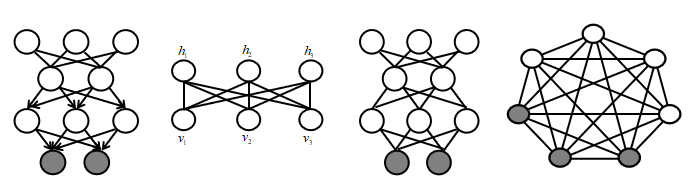
\includegraphics[width=.9\textwidth]{微信图片_20200521215417.png}
    \caption{四种玻尔兹曼机的概率图模型}
    \label{fig:my_label_1}
\end{figure}
显然,深度玻尔兹曼机和深度信念网络的区别就仅仅在于有向和无向上。其中,RBM,DBM和BM都是玻尔兹曼机,而DBN和玻尔兹曼机就不太一样,实际上是一个混合模型,最上面是RBM,而下面的部分都是有向图。

\section{Boltzmann Machine的发展历史}
\subsection{Boltzmann Machine}
最早于1983年诞生的是BM,其概念是来源于Hopfield Network,这个Hopfield Network来源于统计物理学中的Ising Model。看来,机器学习和统计物理还挺有缘的,记得前面见过的吉布斯分布(玻尔兹曼分布)吗,也是来源于统计物理学,包括强化学习中的很多概念也是。BM提出了以后就给出了learning rules。Learning rules就是一个简单的随机梯度上升(Stochastic Gradient Ascend,SGA),SGA的学习规则为:
\begin{equation}
    \triangle w_{ij} = \alpha \left[ \underbrace{\mathbb{E}_{P_{\text{data}}}[v_ih_j]}_{\text{Postive phase}} - \underbrace{\mathbb{E}_{P_{\text{model}}}[v_ih_j]}_{\text{Negative phase}} \right]
\end{equation}
\begin{equation}
    \left\{
    \begin{array}{ll}
      P_{\text{data}} = P_{\text{data}}(v,h) = P_{\text{data}}(v) \cdot P_{\text{model}}(h|v) & \\
      P_{\text{model}} = P_{\text{model}}(v,h) & \\
    \end{array}
    \right.
\end{equation}
其中,$P_{\text{data}}(v)$表示由$N$个样本组成的经验分布,就是我们的数据,而$P_{\text{model}}(h|v)$是由模型得出的后验分布,$P_{\text{model}}(v,h)$是联合概率分布,也就是模型本身。分布的计算都是通过MCMC采样来完成的,其缺点也很明显,就是无法解决过于复杂的问题,很容易遇到收敛时间过长的问题。所以,后来为了简化模型,提出了只有两层的RBM模型。

\subsection{Restricted Boltzmann Machine}
RBM模型相对比较简单。但是Hinton老爷子当时不以为然,觉得RBM模型太简单了,表达力不够好。并于2002年,提出了对比散度(CD)算法,这个算法在之前的“直面配分函数”那章已经做了非常详细的介绍。基于对比散度的采样,实际上就是变了形的Gibbs采样,牺牲了部分精度来提高效率,核心目的就是让采样更加高效。同时,CD算法也给了普通的Boltzmann机的学习算法一些借鉴。然后,后续又发展出了概率对比散度(PCD),一种变形的对比散度,采用的Variational inference来对$P_{\text{model}}(v,h)$进行近似,从而RBM的Learning问题可以得到有效的解决方式,有兴趣的同学可以自己查阅。

\subsection{Deep Belief Network}
因为,RBM的表达能力较弱,所以最简单的思路就是通过叠加多个RBM来增加其层数,从而增加表达能力。但是,增加层数得到的不是Deep Boltzmann Machines,而是Deep Belief Network,具体请详细阅读“深度信念网络”。DBN虽然预训练上是叠加两个RBM而成,但是表现形式并不是玻尔兹曼机。又因为其不是玻尔兹曼机,所以不能用(Stochastic Gradient Ascend,SGA)法来解决。DBN的求解思路为:
$$
\left\{
\begin{array}{ll}
      \text{Pre-training (Staking RBM)} & \\
      \text{Fine-training} \left\{
      \begin{array}{ll}
          \text{Wake-Sleep 无标签} &  \\
          \text{BP 有标签} & 
      \end{array} \right.& \\
\end{array}
\right.
$$
算法需要求解的是每一层的权值。第一步则是通过预训练来得到每层的初始值。在后续的Fine-training中,无标签的情况等价于Wake-Sleep算法求解,如果有标签的话大家觉得是不是和神经网络很像,采用BP算法求解。

\subsection{Deep Boltzmann Machine}
2008年以后,诞生了Deep Boltzmann Machine,显然这与DBN有很大的不同之处。在之前介绍的解决Boltzmann Machines的SGA算法,不能解决大规模处理的问题,在DBM的求解中的能力大打折扣。很多研究者都想找到高效的learning rules。其中较好的想法是,先通过预训练来找到一些比较好的权值,然后再使用SGA。大致流程可做如下描述:
$$
\left\{
\begin{array}{ll}
      \text{Pre-training (Staking RBM)} & \\
      \text{SGA} & \\
\end{array}
\right.
$$
如果没有这个预训练的话,效果非常的不好,时间非常的长。因为,权值的初始值没有任何参考,直接就训练太弱了。关于DBM的联合训练方法,就是不通过预训练的方法,这章不作过多介绍。

\subsection{小结}
本小节介绍了四种Boltzmann machine的发展各自的优缺点等。下一小节主要介绍Hinton提出的权值初始化预训练的方法,如何将一层层的RBM进行叠加得到最终的DBM,并介绍其与DBN中的预训练有什么不一样。

\section{预训练}
\subsection{DBN中RBM结合方法的缺陷}
预训练这一章介绍的是,如何叠加两个RBM,DBN和DBM的不同之处在于如何融合不同的RBM。实际上DBN和DBM的每一层的训练都是一样的,唯一的不同就在于各层训练好之后,如何combine。首先回顾一下RBM,假如现在只有一层,其他层我们都不考虑:
\begin{figure}[H]
    \centering
    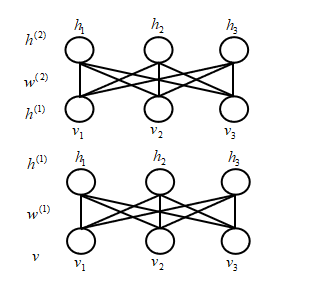
\includegraphics[width=.4\textwidth]{微信图片_20200523155106.png}
    \caption{限制玻尔兹曼机的概率图模型}
    \label{fig:my_label_1}
\end{figure}
首先,哪些是已知的呢?数据的分布$P_{\text{data}(v)}$是知道的。那么在每一步迭代过程中,可以求出Log-Likelihood梯度,利用对比散度采样(CD-K)算法,就可以把$w^{(1)}$学习出来,而且学习到的$w^{(1)}$还不错,当然这个只是近似的,精确的求不出来,主要原因是后验分布是近似采样得到的。有关RBM的参数学习在“直面配分函数”那章,已经做了详细的描述,这里不再多说了。

我们来表达一下这个模型:
\begin{equation}
    \begin{split}
        P(v) = & \sum_{h^{(1)}} P(h^{(1)},v) = \sum_{h^{(1)}} P(h^{(1)})P(v|h^{(1)}) \\
        = & \sum_{h^{(1)}} P(h^{(1)};w^{(1)})P(v|h^{(1)},w^{(1)}) \\
    \end{split}
\end{equation}
其中参数是$w^{(1)}$,为什么呢?因为$P(h^{(1)}) = \sum_v P(v,h)$,而$v$和$h$之间显示是靠$w^{(1)}$来连接的,所以$P(h^{(1)})$一定是和$w^{(1)}$相关的。

第一个RBM求出来以后,那么第二个RBM怎么求呢?实际上这里的$h^{(1)}$都是我们假设出来的。那么下一层RBM连样本都没有,怎么办呢?我们可以将$h^{(1)}$当成是下一个RBM的样本,那么采样得到$h^{(1)}$好采吗?当然简单啦!我们要求的分布为:
$$
P(h^{(1)}|v;w^{(1)})
$$
其中,$v,w^{(1)}$都是已知的,而且由于RBM的良好性质,$h^{(1)}$的节点之间都是相互独立的,那么:
\begin{equation}
    P(h^{(1)}|v;w^{(1)}) = \prod_{i=1}^3 P(h^{(1)}_i|v;w^{(1)})
\end{equation}
而$P(h^{(1)}_i=1|v;w^{(1)}) = \sigma(\sum_{j=1}^3 w_{ij}v_j)$,而$P(h^{(1)}_i=0|v;w^{(1)}) = 1 -  \sigma(\sum_{j=1}^3 w_{ij}v_j)$,既然概率值我们都算出来了,从0/1分布中采样实在是太简单了。

~\\

现在,已经将$h^{(1)}$作为下一层RBM的样本,那么怎么构造$h^{(2)}$呢?我们这样构造,
$$
P(h^{(1)};w^{(2)}) = \sum_{h^{(2)}}P(h^{(1)},h^{(2)};w^{(2)})
$$
DBM中把两个RBM简单的挤压成了一个,这个挤压方式很简单,就是用$P(h^{(1);w^{(2)}})$来代替$P(h^{(1);w^{(1)}})$,为什么呢?因为,公式(3)的主要难点是要得到$P(h^{(1)})$的概率分布,通过加一层的方式,用第二个RBM来对$P(h^{(1)})$进行建模,这时替换过后$P(h^{(1)})$是和$w^{(2)}$相关了,而公式(3)中是和$w^{(1)}$相关的。这样对$h^{(1)}$进行建模时,只用到了一层的权重。而大家想想真实的$P(h^{(1)})$到底和什么有关,写出来就知道了:
$$
P(h^{(1)}) = \sum_{v,h^{(2)}} P(h^{(1)},h^{(2)},v)
$$
看到这个公式,用屁股想都知道肯定和$w^{(1)}$和$w^{(2)}$都有关。所以,应该表达为$P(h^{(1)};w^{(1)},w^{(2)})$。那么,这样直接压缩的方式是有问题的,DBN采用的就是这种方法(箭头怎么来的,不解释了,“深度信念网络”那一节有详细的解释。),那么DBN中对$h^{(1)}$进行建模时,只用到了一层的权重,
无论用哪一层,肯定是不恰当的。

那么,这样就给了我们一个启示,可不可以同时用到$P(h^{(1)};w^{(1)})$和$P(h^{(1)};w^{(2)})$,对他们两做一个平均,就没有那么极端。简单的处理 就是取一个平均数就可以了。

{\color{red}启发:用$P(h^{(1)};w^{(1)})$和$P(h^{(1)};w^{(2)})$几何平均近似$P(h^{(1)};w^{(1)},w^{(2)})$,这样肯定更加适合,但是怎么平均,是简单的相加除2吗?后续会详细的说明。}

\subsection{Double counting problem}
真正要求的是:$P(h^{(1)};w^{(1)},w^{(2)})$。

而目的的直觉是:用$P(h^{(1)};w^{(1)})$和$P(h^{(1)};w^{(2)})$几何平均近似$P(h^{(1)};w^{(1)},w^{(2)})$。

\begin{figure}[H]
    \centering
    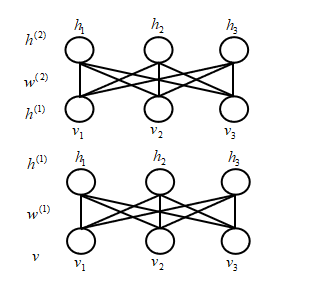
\includegraphics[width=.4\textwidth]{微信图片_20200523155106.png}
    \caption{限制玻尔兹曼机的概率图模型}
    \label{fig:my_label_1}
\end{figure}

其中,
$$
\left\{
\begin{array}{ll}
       P(h^{(1)};w^{(1)}) = \sum_v P(v, h^{(1)};w^{(1)}) = \sum_v P(v)P( h^{(1)}|v;w^{(1)}) & \\
        P(h^{(1)};w^{(2)}) = \sum_{h^{(2)}} P( h^{(1)},h^{(2)};w^{(2)}) = \sum_{h^{(2)}} P(h^{(2)})P( h^{(2)}|h^{(1)};w^{(1)})
\end{array}
\right.
$$
模型中真实存在的只有$v$,而$h^{(1)}$实际上是不存在的,这是我们假设出来的。上一小节讲到了DBN的结合两个RBM的思路中,用$w^{(2)}$来代替$w^{(1)}$,只用到了一层参数。换句话说,只用$P(h^{(1)};w^{(2)})$来近似真实的$P(h^{(1)};w^{(1)},w^{(2)})$,而舍弃了$P(h^{(1)};w^{(1)})$。很自然的可以想到,想要结合$P(h^{(1)};w^{(1)})$和$P(h^{(1)};w^{(2)})$,那么下一个问题就是怎么结合?

实际上,$\sum_v P(v)P( h^{(1)}|v;w^{(1)})$这个分布我们是求不出来的。通常是用采样的方法近似求解,假设观测变量集合为:$v\in V,|V|=N$。那么有:
\begin{equation}
    \begin{split}
        \sum_v P(v)P( h^{(1)}|v;w^{(1)}) = & \mathbb{E}_{P(v)}[P( h^{(1)}|v;w^{(1)})] \\
        \approx & \frac{1}{N} \sum_{v\in V} P(h^{(1)}|v;w^{(1)})
    \end{split}
\end{equation}
其中,$\frac{1}{N} \sum_{v\in V} P(h^{(1)}|v;w^{(1)})$也被称为Aggregate Posterior(聚合后验),代表着用$N$个样本来代替分布。同样,关于$\sum_{h^{(2)}} P( h^{(1)},h^{(2)};w^{(2)})$可以得到:
\begin{equation}
    \sum_{h^{(2)}} P( h^{(1)},h^{(2)};w^{(2)}) \approx
    \frac{1}{N} \sum_{h^{(2)}\in H} P(h^{(2)}|h^{(1)};w^{(2)})
\end{equation}
然后,$N$个$h^{(1)}$再根据$w^{(2)}$采样出$N$个$h^{(2)}$,实际上,在learning结束之后,知道$w^{(1)}$和$w^{(2)}$的情况下,采样是很简单的。这样,从底向上采样,就可以计算出各层的后验,合并很简单:
\begin{equation}
\frac{1}{N} \sum_{v\in V} P(h^{(1)}|v;w^{(1)}) +   \frac{1}{N} \sum_{h^{(2)}\in H} P(h^{(2)}|h^{(1)};w^{(2)})  
\end{equation}
即可。这样采样看着倒还是很合理的,那么到底好不好呢?有什么样的问题呢?

这样会导致,Double Counting的问题,也就是重复计算。

假设$V:$是样本集合,$v\in V$;$H:$才是样本集合,$h^{2}\in H$。采样是从下往上依次进行采样,所以,$h^{1},h^{2}$都依赖于$v$。所以,在计算$h^{1},h^{2}$的过程中都用到了$v$相当于把样本利用了两次。那么,重复计算会带来怎样的副作用呢?

下面举一个例子:
\begin{figure}[H]
    \centering
    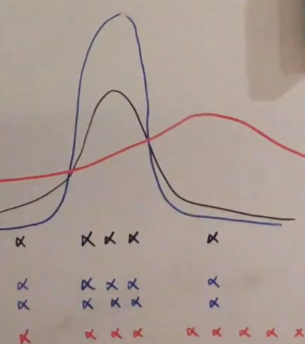
\includegraphics[width=.3\textwidth]{微信图片_20200523152628.png}
    \caption{double counting问题举例}
    \label{fig:my_label_1}
\end{figure}

假如红色的是真实分布,我们实际采样得到的是黑色的样本。简单的假设为高斯分布,利用极大似然估计得到黑色的分布。然后不同的利用黑色的样本,从中采样,采样结果重合,不停的重复利用,会导致所表达的分布越来越尖。从而使得偏差很大,所以简单的结合并不行。

\subsection{预训练总结}
上一小节,我们介绍了double counting问题。实际上在玻尔兹曼机这个系列中,我们可以计算的只有RBM,其他版本的玻尔兹曼机我们都搞不定。所以,就想办法可不可以将RBM叠加来得到具有更好的表达能力的RBM模型,于是第一次简单尝试诞生的就是DBN,DBN除了顶层是双向的,其他层都是单向的。中国武学中讲究“任督二脉”,DBN就像只打通了一半,另一半是不通的。很自然,我们想把另外一半也打通,这么模型的表示能力就更强一些。
\begin{figure}[H]
    \centering
    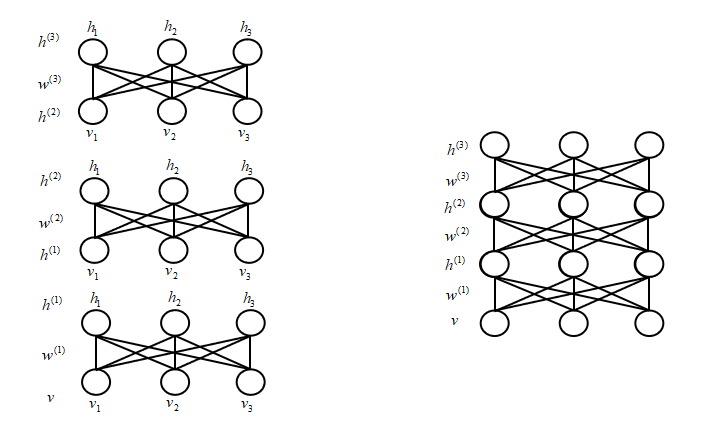
\includegraphics[width=.8\textwidth]{微信图片_20200523155948.png}
    \caption{利用分层训练RBM得到DBM的参数}
    \label{fig:my_label_1}
\end{figure}
那么,最开始就是将每层RBM的参数$w^{(1)}$,$w^{(2)}$,$w^{(3)}$训练出来之后分别赋予DBM中的$w^{(1)}$,$w^{(2)}$,$w^{(3)}$。但是,这样就会有只用到了一层的参数,所以解决方案是取平均值。比如,在分层的RBM训练中,求的是$2w^{(1)}$,$2w^{(2)}$,$2w^{(3)}$,再将权值$w^{(1)}$,$w^{(2)}$,$w^{(3)}$赋予DBM,相对于每一次只用到了一半的权重。那么,对于中间层$h^{(1)}$来说,就相对于同时用到了$w^{(1)}$,$w^{(2)}$这个在前面,我们已经详细的讲过了。

然而,问题又来了,$v$和$h^{(3)}$只和一层相连。那么,除以2感觉上有一些不对。给出的处理方法是,在RBM的分层学习中,对于$v$从上往下是$w^{(1)}$,从下往上是$2w^{(1)}$,这个问题就解决了。这时不是一个简单的RBM了,我们称之为“RBM”,哈哈哈哈。其近似的概率图模型可以这样认为,来帮助我们理解:
\begin{figure}[H]
    \centering
    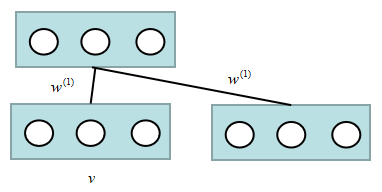
\includegraphics[width=.6\textwidth]{微信图片_20200523162935.png}
    \caption{利用分层训练RBM得到DBM的参数}
    \label{fig:my_label_1}
\end{figure}
那么,进到$h^{(1)}$有两个$w^{(1)}$,也就是$2w^{(1)}$,而进到$v$只有一个$w^{(1)}$。这就等价于从上往下是$w^{(1)}$,从下往上是$2w^{(1)}$。除了,第一层和最后一层,其他层的都是学习的两倍权值,第一层和最后一层则是“RBM”。

从直觉上看,感觉这一系列演变会让模型的性能越来越好。实际上,可以通过数学证明,DBM的ELBO、比DBN要高,而且DBM的层数越多,每叠加一层RBM,ELBO都会更高。

\section{本章小结}
这章中比较完善的讲解了DBM,通过将DBM拆解为若干个RBM,然后对RBM进行分层的来进行预训练,并将其预训练得到的权重直接赋予DBM的方法。实际上,这只是最经典的训练DBM的方法,近些年诞生了很多直接训练的方法,效果也很不错,现在基本也没有人用预训练了。但是,这种基本思想还是很值得学习的。

本章的主要内容,介绍了四种玻尔兹曼模型的发展,并重点介绍了DBN模型的不足之处(对中间层建模用到一层的参数),从而引出了DBM模型;介绍了DBM模型中的Double counting问题,并对其进行了详细的解释;最后对DBM模型进行了总结,并解释了边界层的处理方法。

实际上DBM模型的演变都非常的Intuitive,不需要太多的数学证明也可以理解。个人觉得这样的思想在科研中很重要,很多情况都是有一个intuitive的想法,然后实验发现确实work,最后寻找证明的方法。(个人愚见)


\end{document}
